\section*{Цель работы.}
Изучение функций и способов обработки массивов данных, а также способов форматированного вывода информации.

\section*{Задания.}
\begin{enumerate}
    \item В соответствии с таблицей 1 создать матрицы, содержащие сетку аргументов и значения поверхности.
    \item Задать с клавиатуры значение уровня поверхности.
    \item Найти и вывести в командное окно 10 точек, звначение в которых превышает заданный уровень поверхности.
    \item Построить поверхность функции $f(x_1,x_2)$, ограниченной заданным уровнем.
    \item По любой из точек из п. 3 сформировать одномерные массивы аргумента (в соответствии с заданием преподавателя) и проекции поверхности.
    \item Определить диапазон (диапазоны), в котором проекция превышает уровень поверхности, заданный в п. 2. Выполнить для этого диапазона операцию отражения или растяжения (рисунок 2), в соответствии с заданием преподавателя. Построить графики исходной и обработанной проекции.
    \item Ввести строку данных с клавиатуры согласно прототипу (\cref{table:ex7}). Обеспечить считывание данных из строки. Вывести переменные и значения на экран.
\end{enumerate}

\section*{Требования к выполнению заданий.}
\begin{enumerate}
    \item Графики обработанной поверхности и проекции (задания 4, 5, 6) должны выводиться в разных окнах.
    \item В отчете должна быть приведена формула отражения / растяжения (задание 6).
    \item В отчете должно быть приведено описание функций работы со строками/символами, которые будут использованы при выполнении задания (задание 7).
\end{enumerate}


\section*{Экспериментальные результаты.}
\section*{ \boxed{\text{ Задание 1. }} }

\begin{quote}
    \textit{В соответствии с таблицей 1 создать матрицы, содержащие сетку аргументов и значения поверхности.}
\end{quote}

\begin{table}[H]
    \centering
    \caption{Формула для 3 варианта}
    \label{table:ex1}
    \begin{tabular}{cc}
            Функция $f(x_1, x_2)$ & Диапазон \\
        \toprule
            $ (x_1^2 - 10\cos(2\pi x_2)) (x_2^2-10\cos\left(\frac{2\pi x_1}{5}\right)) $ & $x_i\in[-5; 5]$
    \end{tabular}
\end{table}

\begin{listing}[H]
    \caption{Исходный график}
    \label{lst:Исходный график}
    \inputminted[
        % firstline=7,
        % lastline=10,
        % highlightlines={1-10},
    ]{matlab}{code/ex1.m}
\end{listing}

\section*{ \boxed{\text{ Задание 2. }} }
\begin{quote}
    \textit{Задать с клавиатуры значение уровня поверхности.}
\end{quote}

\begin{listing}[H]
    \caption{Получение значения плоскости сечения}
    \label{lst:Получение значения плоскости сечения}
    \inputminted[
        % firstline=16,
        % lastline=17,
        % highlightlines={1-10},
    ]{matlab}{code/ex2.m}
\end{listing}

\section*{ \boxed{\text{ Задание 3. }} }
\begin{quote}
    \textit{Найти и вывести в командное окно 10 точек, звначение в которых превышает заданный уровень поверхности. }
\end{quote}

Вывод точек поверхности должен осуществляться в виде: $f(x_1, x_2) = value$. Решение данной задачи представлено в двух вариантах: с использованием функции \textit{find} (см. \cref{lst:with_find}) и без её использования (см. \cref{lst:without_find}).

\begin{listing}[H]
    \caption{Поиск 10 наиб. знач. огр. верхнего графика (с использования функции \textit{find})}
    \label{lst:with_find}
    \inputminted[
        % firstline=23,
        % lastline=28,
        % highlightlines={1-10},
    ]{matlab}{code/ex3_with_find.m}
\end{listing}

Строки 5 и 6 таковы, что в \mintinline{x}!Z_up_slice! попадают только те значения, которые превышают уровень сечения \mintinline{x}!slice!, а все значения ниже уровня сечененя заменяются на \textit{NaN}. 
Соотв. в \mintinline{x}!Z_down_slice! попадают все остальные значения (ниже уровня сечения). 
При этом обрезанные шапки выравниваются со значением \mintinline{x}!slice!, график имел более эстетичный вид.

\begin{listing}[H]
    \caption{Поиск 10 наиб. знач. огр. верхнего графика (без использования функции \textit{find})}
    \label{lst:without_find}
    \inputminted[
        % firstline=23,
        % lastline=48,
        % highlightlines={1-10},
    ]{matlab}{code/ex3_without_find.m}
\end{listing}

Результат работы программ представлен на \cref{fig:ex3}. Для вывода данных используются флаги \mintinline{regex}!\t!, \mintinline{regex}!\n!. Первый означает знак табуляции (в данной задаче он нужен для равного расстояния между числами). Второй знак является знаком новой строки.

\begin{figure}[H]
    \centering
    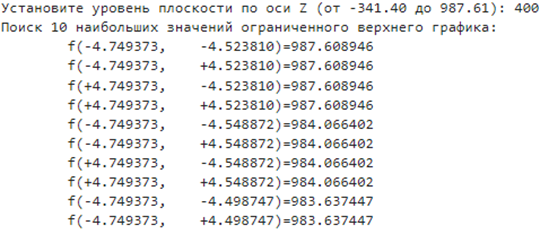
\includegraphics[width=0.7\textwidth]{figs/ex3.png}
    \caption{Результат работы поиска 10 наиб. знач.}
    \label{fig:ex3}
\end{figure}

\section*{ \boxed{\text{ Задание 4. }} }
\begin{quote}
    \textit{Построить поверхность функции $f(x_1,x_2)$, ограниченной заданным уровнем. }
\end{quote}

\begin{listing}[H]
    \caption{Отображение графиков}
    \label{lst:Отображение графиков}
    \inputminted[
        % firstline=53,
        % lastline=79,
        % highlightlines={1-10},
    ]{matlab}{code/ex4.m}
\end{listing}

Примечательно, что в программе есть переменная \mintinline{x}!showFigures!, которая по умолчанию равна \mintinline{x}!true!.
Её наличие в программе обусловлено тем, что при отладке программы иногда требуется отключать отображение графиков, чтобы не мешать работе.

Результат работы программы представлен далее:
\begin{figure}[H]
    \centering

    \begin{subfigure}{0.48\textwidth}
        \centering
        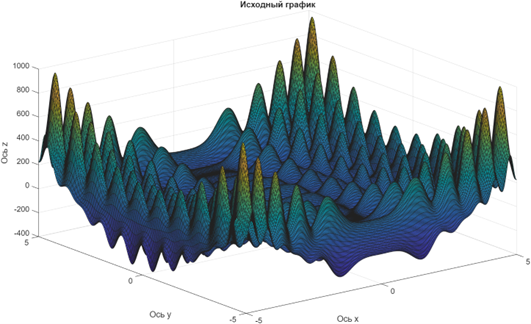
\includegraphics[width=\linewidth]{figs/ex4_1.png}
        \caption{Исходный график}
        \label{fig:Исходный график}
    \end{subfigure}
    \hfill
    \begin{subfigure}{0.48\textwidth}
        \centering
        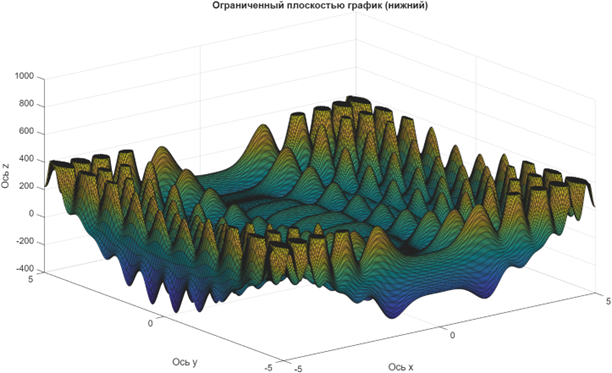
\includegraphics[width=\linewidth]{figs/ex4_2.png}
        \caption{Ограниченный плоскостью}
        \label{fig:Ограниченный плоскостью}
    \end{subfigure}

     \caption{Демонстрация графиков}
    \label{fig:graphics_demo}
\end{figure}

\section*{ \boxed{\text{ Задание 5. }} }
\begin{quote}
    \textit{По любой из точек из п. 3 сформировать одномерные массивы аргумента (в соответствии с заданием преподавателя) и проекции поверхности.}
\end{quote}

\begin{listing}[H]
    \caption{Случайная точка из п.3 и проекция поверхности}
    \label{lst:Случайная точка из п.3 и проекция поверхности}
    \inputminted[
        % firstline=84,
        % lastline=114,
        % highlightlines={1-10},
    ]{matlab}{code/ex5.m}
\end{listing}

Результат работы программы представлен далее:
\begin{figure}[H]
    \centering
    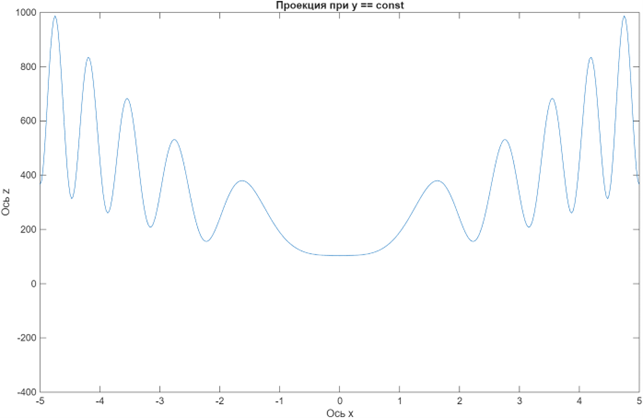
\includegraphics[width=0.5\textwidth]{figs/ex5.png}
    \caption{Проекция при $y=const$}
    \label{fig:Проекция при $y=const$}
\end{figure}

\section*{ \boxed{\text{ Задание 6. }} }
\begin{quote}
    \textit{Определить диапазон (диапазоны), в котором проекция превышает уровень поверхности, заданный в п. 2. Выполнить для этого диапазона операцию отражения или растяжения (рисунок 2), в соответствии с заданием преподавателя. Построить графики исходной и обработанной проекции. }
\end{quote}

\begin{figure}[H]
    \centering
    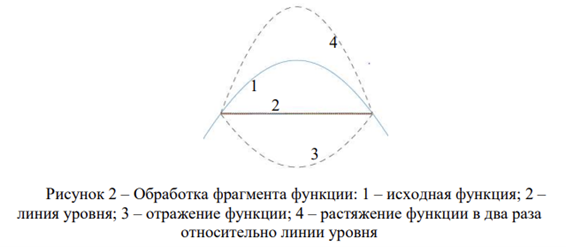
\includegraphics[width=0.8\textwidth]{figs/ex6.png}
    % \caption{caption}
    \label{fig:условия задания}
\end{figure}

\begin{listing}[H]
    \caption{Работа с диапазонами над плоскостю сечения}
    \label{lst:Работа с диапазонами над плоскостю сечения}
    \inputminted[
        % firstline=120,
        % lastline=158,
        % highlightlines={1-10},
    ]{matlab}{code/ex6.m}
\end{listing}


\begin{figure}[h!]
    \centering

    % --- Верхний ряд ---
    \begin{subfigure}{0.48\textwidth}
        \centering
        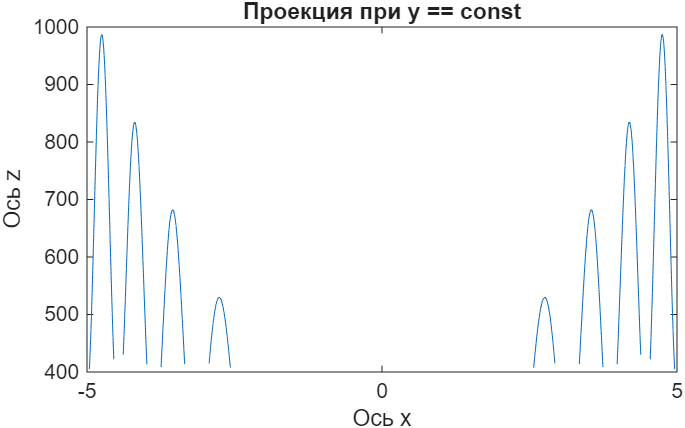
\includegraphics[width=\linewidth]{figs/ex6_1.png}
        \caption{Проекция при $y=\text{const}$}
        \label{fig:ex6_1} % Используйте простые метки
    \end{subfigure}
    \hfill % Разделитель между изображениями в ряду
    \begin{subfigure}{0.48\textwidth}
        \centering
        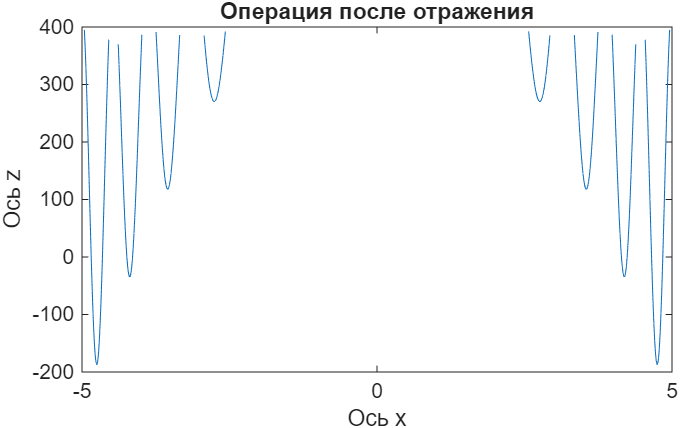
\includegraphics[width=\linewidth]{figs/ex6_2.png}
        \caption{Операция отражения}
        \label{fig:ex6_2}
    \end{subfigure}

    \vspace{0.5cm} % Вертикальный отступ между рядами

    % --- Нижний ряд ---
    \begin{subfigure}{0.48\textwidth}
        \centering
        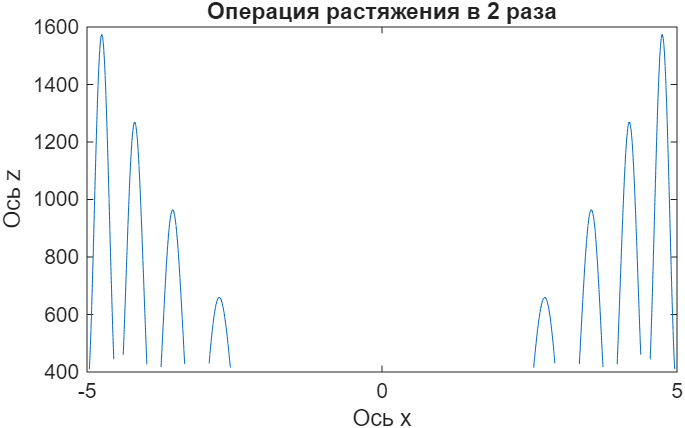
\includegraphics[width=\linewidth]{figs/ex6_3.png}
        \caption{Операция растяжения в два раза}
        \label{fig:ex6_3}
    \end{subfigure}
    \hfill % Разделитель между изображениями в ряду
    \begin{subfigure}{0.48\textwidth}
        \centering
        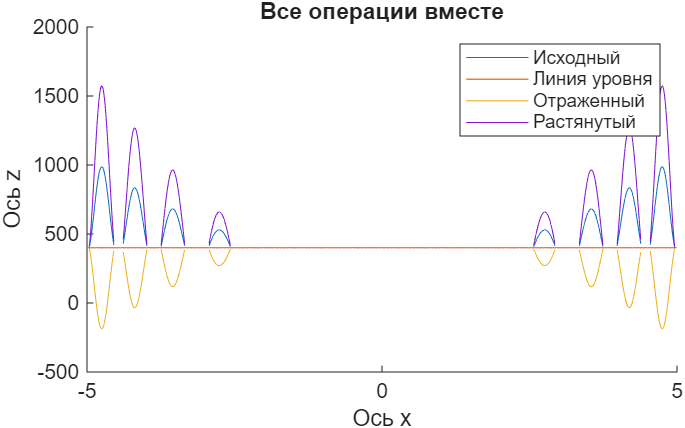
\includegraphics[width=\linewidth]{figs/ex6_4.png}
        \caption{Все операции вместе}
        \label{fig:ex6_4}
    \end{subfigure} % Опечатка в вашем коде, должно быть subfigure

    % --- Общая подпись (если нужна) ---
    \caption{Демонстрация последовательных операций над графиком}
    \label{fig:all_operations}
\end{figure}

Формулы отражения и растяжения соотв.:
$$f(x) = -f(x) + 2s,$$
$$f(x) = 2 * f(x) - s,$$
где $f(x)$ --- \mintinline{x}!projection_array!, $x$ --- \mintinline{x}!slice! (линия уровня).

\section*{ \boxed{\text{ Задание 7. }} }
\begin{quote}
    \textit{Ввести строку данных с клавиатуры согласно прототипу (\cref{table:ex7}). Обеспечить считывание данных из строки. Вывести переменные и значения на экран.}
\end{quote}

\begin{table}[H]
    \centering
    \caption{Прототип символьных сообщения для 3 варианта}
    \label{table:ex7}
    \begin{tabular}{cc}
            Прототип & Тип данных \\
        \toprule
            \mintinline{regex}!#array#:name: _val1 _val2 _val3 ...#endarray#! & \textit{char}
    \end{tabular}
\end{table}

\begin{listing}[H]
    \caption{Вывод данных}
    \label{lst:Вывод данных}
    \inputminted[
        % firstline=157,
        % lastline=179,
        % highlightlines={1-10},
    ]{matlab}{code/ex7.m}
\end{listing}

\begin{figure}[H]
    \centering
    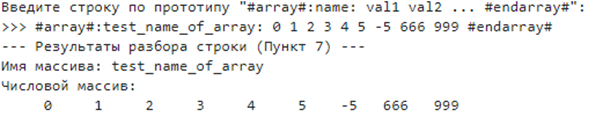
\includegraphics[width=0.8\textwidth]{figs/ex7.png}
    \caption{Результат выполнения задания 7}
    \label{fig:Результат выполнения задания 7}
\end{figure}

Принцип работы чтения введённой пользователем строки заключается в использовании технологии regex. Она имеет следующие особенности работы в MatLab.

Все используемые поля следует именовать: \textit{(?<xxx>yyy)}, где \textit{( )} — ограничители поля; \textit{xxx} — имя поля, по которому будем осуществляться обращение в получившейся структуре в коде MatLab; \textit{yyy} — ключи для считывания строки.

\begin{itemize}
    \item Ключ \mintinline{matlab}!\w! означает считывание любого строчного символа (включая знак \mintinline{matlab}!_!).
    \item Ключ \mintinline{matlab}!+! означает «1 и более». В совокупности с ключом \mintinline{matlab}!\w! будет означать «1 и более символ».
	\item Ключ \mintinline{regex}![^ #]!. Квадратные скобки позволяют объявить пользовательский набор символов. Знак \mintinline{matlab}!^! считывается как «до» (не включительно). Таким образом данный ключ можно считать как «все символы до символа решетки не включительно».
\end{itemize}
	
После считывания строки происходит её обработка. В функции \textit{regexp} обрабатывается введённая пользователем строка \textit{input\_str} по паттерну \textit{pattern} с флагом \textit{‘names’} (который диктует наличие именованных полей в паттерне), таким образом создавая структуру \textit{tokens}.

Затем происходит обращение к полям данной структуры для дальнейшей обработки данных. Так, например, введённые \textit{val1}, \textit{val2}, ..., \textit{valn} разделяются по знаку пробела и преобразуются в числовой тип данных \textit{double} функцией \textit{str2double}. Функцией \textit{isnan} находится нечисловые данные и удаляются (такое может происходить, если пользователь ввёл лишние пробелы).

\section*{Выводы.}

Были решены все задачи. Цель лабораторной работы была успешно достигнута, продемонстрировав владение методами векторизованной обработки числовых и символьных массивов в MATLAB. 